\documentclass{article}
\usepackage{caption}
\usepackage{graphicx}
\begin{document}
\fbox{ 
{\centering
\begin{minipage}{0.30\textwidth}
  \centering
  
	\begin{center}
	\begin{tabular}{ |c|c| } 
 	\hline
 		Item&Value\\ \hline\hline
 		a &  .99  	\\ \hline
 		b &  .54   	\\ \hline
 		
\end{tabular}
\end{center}  

  
  \captionof{table}{Header }
\end{minipage}
  \hfill
\hfill
\begin{minipage}{0.29\textwidth}
  \centering
  \hfill
  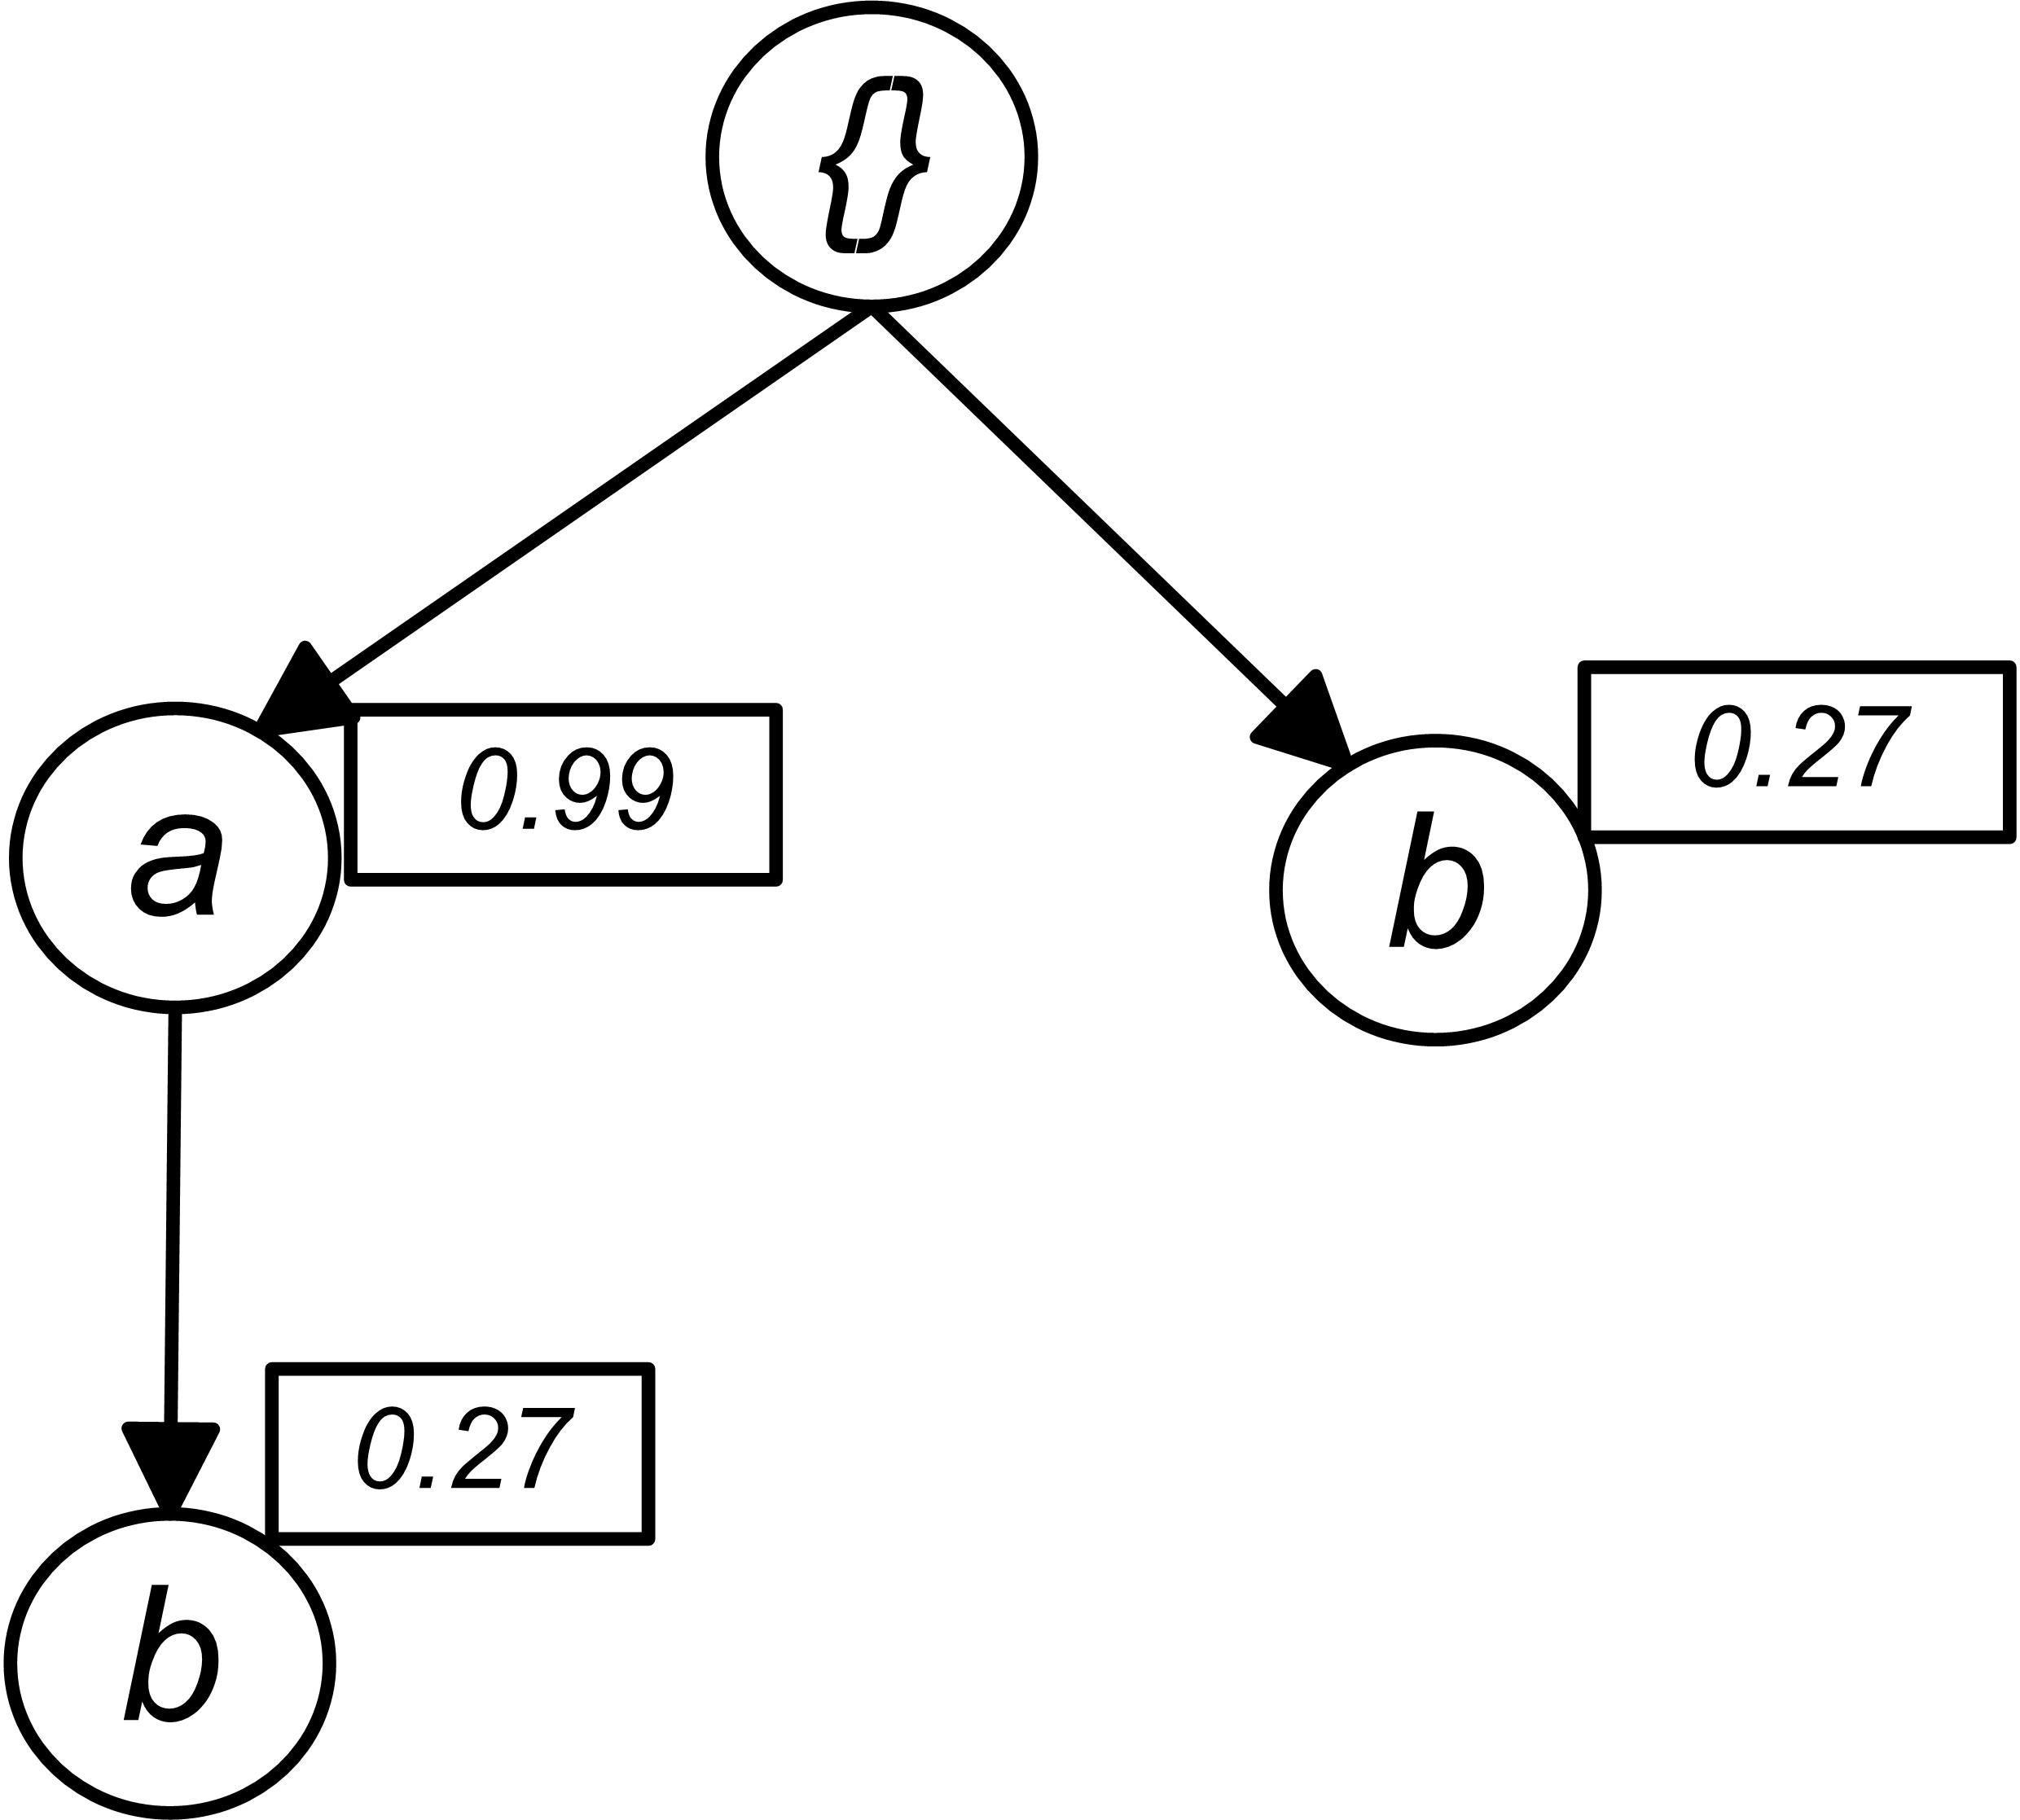
\includegraphics[width=.8\textwidth, height=3.5cm]{../images/C_COND.jpg}
  \captionof{figure}{\emph{c-cond Tree}}
  \hfill
  
\end{minipage}
\hfill
\begin{minipage}{0.30\textwidth}
  \centering
  
	\begin{center}
	\begin{tabular}{ |c| } 
 	\hline
 		Freq Patterns \\ \hline\hline
 		ca  	\\ \hline
 		
\end{tabular}
\end{center}  

  
  \captionof{table}{ \emph{Freq Patterns} }
\end{minipage}
}
}

\end{document}
